\documentclass[usenames,dvipsnames]{beamer}
%-------------------------------------------------------
% THEME SETTINGS
%-------------------------------------------------------
\usetheme[progressstyle=movingCircCnt]{Feather}
\setbeamercolor{Feather}{fg=black!30,bg=black}
\setbeamercolor{structure}{fg=black}
\setbeamercolor{block body example}{bg=black!5!white}
\setbeamercolor{block title example}{fg=white,bg=black!40!white}


\usepackage{amsmath,amssymb,amsfonts}
\usepackage{cite}
\usepackage{multirow}
\usepackage{booktabs}
\usepackage{hhline}
\usepackage{multicol}
%\usepackage{showframe}

\usepackage{tikz}
%\usetikzlibrary{patterns}
\usetikzlibrary{patterns,arrows,decorations.pathmorphing,backgrounds,shadows,positioning,fit,shapes,matrix,calc,shapes.multipart,arrows.meta}
\usepackage[simplified]{pgf-umlcd}
\usepackage{xpatch} % Needed for patching pgf-umlcd
\usepackage{xparse} % Needed for patching pgf-umlcd
\usepackage{color,soul} % for \hl
\definecolor{dark-yellow}{RGB}{219, 212, 143}
\definecolor{dark-green}{RGB}{36,84,36}
\definecolor{my-gray}{gray}{0.85}
\sethlcolor{dark-yellow}



\usepackage{wrapfig}
\usepackage{listings}
\usepackage{adjustbox}
\usepackage{graphicx}
\usepackage{caption}
\usepackage{multirow}
\usepackage{subcaption}
\usepackage{stmaryrd}
\usepackage{hyperref}
\usepackage{float}
\usepackage{textcomp}
\usepackage{tikz-qtree,tikz-qtree-compat}

\newcommand*{\emphColorSlide}[1]{\textcolor{ForestGreen}{\textbf{#1}}}
\newcommand*{\emphSlide}[1]{\textcolor{ForestGreen}{\textbf{#1}}}

\newcommand*{\lowEmph}[1]{\textcolor{NavyBlue}{\textbf{#1}}}
\newcommand*{\subt}{\textcolor{NavyBlue}{\textbf{<:}}}
\newcommand*{\supt}{\textcolor{NavyBlue}{\textbf{:>}}}



\newcommand{\dataflow}{data-flow}
\newcommand{\Dataflow}{Data-flow}
\newcommand{\code}[1]{\texttt{\lstinline[basicstyle=\normalsize\ttfamily,identifierstyle={\normalsize},commentstyle={\normalsize\itshape},keywordstyle={\normalsize\bfseries},ndkeywordstyle={\normalsize},stringstyle={\normalsize\ttfamily},numberstyle={\normalsize}]!#1!}}
\newcommand{\CFG}{CFG}
\newcommand{\intraj}{\emphColorSlide{\textsc{Intra}J}}
\newcommand{\intrajs}{\emphColorSlide{\textsc{IntraJ}}}
\newcommand{\intracfgs}{\emphColorSlide{\textsc{IntraCFG}}}
\newcommand{\jastaddjintraflow}{\textsc{jastaddj-intraflow}}
\newcommand{\jji}{\code{JJI}}
\newcommand{\jastadd}{\textsc{JastAdd}}
\newcommand{\extendj}{\textsc{ExtendJ}}
\newcommand{\cG}{\mathcal{G}}
\newcommand{\cV}{\mathcal{V}}
\newcommand{\cE}{\rightarrowtail}
\newcommand{\cP}{\mathcal{P}}
\newcommand{\cM}{\mathcal{M}}


\newcommand{\mSyn}{\ensuremath{\uparrow}}
\newcommand{\mInh}{\ensuremath{\downarrow}}
\newcommand{\mHOA}{\ensuremath{\rightarrow}}
\newcommand{\mColl}{\ensuremath{\square}}
\newcommand{\mCirc}{\ensuremath{\circlearrowleft}}

\newcommand{\Abase}[1]{\textcolor{ATGsym}{\mbox{\umlcode{#1}}}}
\newcommand{\Asyn}[1]{\textcolor{ATGsym}{\mbox{\mSyn{}\umlcode{#1}}}}
\newcommand{\Ainh}[1]{\textcolor{ATGsym}{\mbox{\mInh{}\umlcode{#1}}}}
\newcommand{\Ahoa}[1]{\textcolor{ATGsym}{\mbox{\mHOA{}\umlcode{#1}}}}
\newcommand{\Acoll}[1]{\textcolor{ATGsym}{\mbox{\mColl{}\umlcode{#1}}}}
\newcommand{\Acirc}[1]{\textcolor{ATGsym}{\mbox{\mCirc{}\umlcode{#1}}}}

\newcommand{\umlcode}[1]{\textrm{#1}}  % Style of code used in UML fragments
\newcommand{\astnodestyle}{\ttfamily\color{magenta}}
\newcommand{\astnode}[1]{\texttt{\textcolor{magenta}{#1}}}  % Style used for AST node types

\newcommand{\ASTUnrestricted}{AST-unrestricted}
\newcommand{\ParentFirst}{Parent-First}

\newcommand{\project}[1]{\textsc{#1}}
\newcommand{\tool}[1]{\textsc{#1}}

% can't get fbox to work reliably in the UML code, and adjustbox and nested \tikz don't work at all
%\newcommand{\dfapi}{\textsf{\setlength{\fboxsep}{0pt}\fcolorbox{blue}{white}{df-api}}}
\newcommand{\dfapi}{\textbf{\textcolor{black}{[df-api]}}}
\newcommand{\nameapi}{\textbf{\textcolor{black}{[name-api]}}}

\newcommand{\frameworkname}{\textsc{Intra}CFG}
\newcommand{\intracfg}{\textsc{\frameworkname}}

\newcommand{\node}{\mathsf{n}}
\newcommand{\Null}{\mathtt{NULL}}
\newcommand{\Notnull}{\mathtt{NOTNULL}}
\newcommand{\gen}{\mathtt{gen}}
\renewcommand{\kill}{\mathtt{kill}}

\newcommand{\In}{\mathtt{in}}
\newcommand{\Out}{\mathtt{out}}
\newcommand{\Use}{\mathtt{use}}
\newcommand{\Def}{\mathtt{def}}
\newcommand{\tf}{f_t}
\newcommand{\mCi}[1]{ { \textcolor{black!30}{\tiny \pm\text{#1}}}}%Condifdence interval

\newcommand{\CR}[1]{\textbf{[}\textcolor{blue!60!black}{\textbf{CR:} #1}\textbf{]}}
\newcommand{\Ckw}[1]{\texttt{\textbf{#1}}}
\newcommand{\auxlabel}[1]{{\scriptsize{$\textrm{\texttt{#1}}$}}}
\newcommand{\auxlabeli}[2]{{\scriptsize{$\textrm{\texttt{#2}}_{#1}$}}}
\newcommand{\auxlabelbox}[1]{\tikz[baseline=-0.7ex] \node[rectangle, minimum width=0, thin, draw, rounded corners, fill=white, inner sep=2pt, outer sep=0pt] (N) {\auxlabel{#1}};}
\newcommand{\auxlabelboxhoa}[1]{\tikz[baseline=-0.7ex] \node[rectangle, dashed,minimum width=0, thin, draw, rounded corners, fill=white, inner sep=2pt, outer sep=0pt] (N) {\auxlabel{#1}};}

%\newcommand{\auxlabelboxi}[2]{\tikz \node[rectangle, minimum width=0, thin, draw, rounded corners, fill=white] {\auxlabeli{#1}{#2}};}

\newcommand{\Prod}{::=}
\newcommand{\terminal}[1]{\textcolor{green!50!black}{\textit{#1}}}
\newcommand{\vmetavar}[1]{\textcolor{cyan!30!black}{\textsf{\textbf{#1}}}}
\newcommand{\vcode}[1]{\textsf{\textcolor{green!35!black}{{#1}}}}
\newcommand{\vterminal}[1]{\vcode{#1}}
\newcommand{\nta}[1]{\ensuremath{\textit{#1}}}
\newcommand{\tuple}[1]{\ensuremath{\langle #1 \rangle}}
\newcommand{\nt}[1]{\ensuremath{\tuple{\hspace{-0.02cm}\nta{#1}\hspace{0.02cm}}}}
\newcommand{\VB}{\ |\ }
\newcommand{\Gcomment}[1]{\textrm{\textcolor{black!50!white}{({#1})}}}
\newcommand{\sem}[1]{\ensuremath{\llbracket #1 \rrbracket}}
%\newcommand{\semNPA}[1]{\ensuremath{\sem{#1}_{\textit{NPA}}}}
\newcommand{\semNPA}[1]{\ensuremath{\sem{#1}}}

\newcommand{\listingsfontsize}{\scriptsize}

\newcommand{\NAmark}{\multicolumn{1}{c}{\textcolor{black!40!white}{-}}}
\newcommand{\NAmarkR}{\multicolumn{1}{c|}{\textcolor{black!40!white}{-}}}
\newcommand{\Tcenter}[1]{\multicolumn{1}{c}{#1}}
\newcommand{\TcenterR}[1]{\multicolumn{1}{c|}{#1}}
\newcommand{\succarrow}{\tikz[baseline=-0.7ex] \draw[succarrow, thick, -{Stealth[scale=0.9, inset=0pt, angle'=45]}] (0,0) -- (0.3,0.0);}

\colorlet{hlgreen}{green}
\colorlet{hlorange}{orange}
\colorlet{hlgreenhalf}{green!50!white}
\colorlet{hlorangehalf}{orange!50!white}
\colorlet{npagrey}{gray!10!white}

\DeclareRobustCommand{\hlgreen}[1]{{\sethlcolor{hlgreenhalf}\hl{#1}}}
\DeclareRobustCommand{\hlorange}[1]{{\sethlcolor{hlorangehalf}\hl{#1}}}

\definecolor{ATGsym}{HTML}{206010}

\definecolor{SQ}{HTML}{0080ff}
\definecolor{JJI}{HTML}{ff0080}
\definecolor{IJnonH}{HTML}{004010}
\definecolor{IJH}{HTML}{00ff20}

\definecolor{succarrow}{HTML}{4e90e2}	% adapted from RunningExample.tex

\definecolor{lightblue}{HTML}{006699}		%#006699
\definecolor{lightgreen}{HTML}{669900}		%#669900
\lstdefinelanguage{JastAdd}{
  %keyword1&2&6
  morekeywords = [1]{class, extends, private, void,new},
  %keyword3
  morekeywords = [2]{this,null}, %JASTADD keywords
  %keyword4
  morekeywords = [3]{return}, %ASTnode typess
  %keyword5
  morekeywords = [4]{},
  keywordstyle = [1]\color{lightblue},
  keywordstyle = [2]\color{lightgreen},
%  keywordstyle = [1]\bfseries,
%  keywordstyle = [2]\bfseries,
  keywordstyle = [3]\astnodestyle,
  keywordstyle = [4]\color{orange},
  sensitive = true,
  morecomment = [l]{//},
  morecomment = [s]{/*}{*/},
  morecomment = [s]{/**}{*/},
  commentstyle = \color{gray},
  morestring = [b]",
  morestring = [b]',
  stringstyle = \color{purple}
}
\lstset{
  backgroundcolor =\color{npagrey},
  basicstyle=\listingsfontsize\ttfamily,
  identifierstyle={\listingsfontsize},
  commentstyle={\listingsfontsize\itshape},
  keywordstyle={\listingsfontsize\bfseries},
  ndkeywordstyle={\listingsfontsize},
  stringstyle={\listingsfontsize\ttfamily},
  frame={tb},
  breaklines=true,
  breakatwhitespace=true, %To avoid linebreaks between \code{} and comma.
  columns=[l]{fullflexible},
  numbers=none,
  numberstyle={\listingsfontsize},
  stepnumber=1,
  mathescape,
	escapeinside     = {!}{!}, %General escape does not seem to work in lstinline/GH.
}

\makeatletter
\pgfdeclareshape{topbottombox}{
  \inheritsavedanchors[from=rectangle]
  \inheritanchorborder[from=rectangle]
  \inheritanchor[from=rectangle]{center}
  \inheritanchor[from=rectangle]{base}
  \inheritanchor[from=rectangle]{north}
  \inheritanchor[from=rectangle]{north east}
  \inheritanchor[from=rectangle]{east}
  \inheritanchor[from=rectangle]{south east}
  \inheritanchor[from=rectangle]{south}
  \inheritanchor[from=rectangle]{south west}
  \inheritanchor[from=rectangle]{west}
  \inheritanchor[from=rectangle]{north west}
  \backgroundpath{
    %  store lower right in xa/ya and upper right in xb/yb
    \southwest \pgf@xa=\pgf@x \pgf@ya=\pgf@y
    \northeast \pgf@xb=\pgf@x \pgf@yb=\pgf@y
    \pgfpathmoveto{\pgfpoint{\pgf@xa}{\pgf@ya}}
    \pgfpathlineto{\pgfpoint{\pgf@xb}{\pgf@ya}}
    \pgfpathmoveto{\pgfpoint{\pgf@xa}{\pgf@yb}}
    \pgfpathlineto{\pgfpoint{\pgf@xb}{\pgf@yb}}
 }
}
\makeatother


% Patch UML package pgf-umlcd to be able to write abstract grammar as class name.
\ExplSyntaxOn
\NewDocumentCommand{\defineclassname}{m}
 {
  \tl_set:Nn \umlcdClassName { #1 }
  \tl_set_eq:NN \umlcdClassNameString \umlcdClassName
  \tl_replace_all:Nfn \umlcdClassName { \char_generate:nn { `_ } { 8 } } { \_\kern1pt }
 }
\cs_generate_variant:Nn \tl_replace_all:Nnn { Nf }
\ExplSyntaxOff
\xpatchcmd{\classAndInterfaceCommon}
 {\def\umlcdClassName}
 {\defineclassname}
 {}{}
\xpatchcmd{\endclass}
 {(\umlcdClassName)}
 {(\umlcdClassNameString)}
 {}{\ddt}
\xpatchcmd{\endinterface}
 {(\umlcdClassName)}
 {(\umlcdClassNameString)}
 {}{\ddt}
\xpatchcmd{\endabstractclass}
 {(\umlcdClassName)}
 {(\umlcdClassNameString)}
 {}{\ddt}
\xpatchcmd{\endobject}
 {(\umlcdClassName)}
 {(\umlcdClassNameString)}
 {}{\ddt}
\xpatchcmd{\endclassAndInterfaceCommon}
 {(\umlcdClassName)}
 {(\umlcdClassNameString)}
 {}{\ddt}
\xpatchcmd{\endclassAndInterfaceCommon}
 {(\umlcdClassName)}
 {(\umlcdClassNameString)}
 {}{\ddt}
\xpatchcmd{\endclassAndInterfaceCommon}
 {(\umlcdClassName)}
 {(\umlcdClassNameString)}
 {}{\ddt}

\newbool{ANON}
%\booltrue{ANON}
\boolfalse{ANON}
\newcommand{\anon}[2]
{\ifbool{ANON}{
   #1
}{
   #2
}}



\makeatletter
\renewcommand\@makefnmark{\hbox{\@textsuperscript{\usebeamercolor[fg]{footnote mark}\usebeamerfont*{footnote mark}[\@thefnmark]}}}
\renewcommand\@makefntext[1]{\@textsuperscript{\usebeamercolor[fg]{footnote mark}\usebeamerfont*{footnote mark}[\@thefnmark]}\usebeamerfont*{footnote} #1}
\makeatother

%Modify the Title display on frame
\makeatletter
\patchcmd\beamer@@tmpl@frametitle{\insertframetitle}{{\footnotesize \insertsection~\emphColorSlide{\insertsubsection}~\\} \textbf{\insertframetitle}}{}{}
\makeatother
%Add space to the footline
\makeatletter
\patchcmd{\beamer@calculateheadfoot}{\advance\footheight by 4pt}{\advance\footheight by 8pt}{}{}
\makeatother

%NO HEAD LINE
\makeatletter
\newenvironment{noheadline}{
	\setbeamertemplate{headline}[default] {}
	\setfootline
}{}
\makeatother

%Slide with  Section title
%\AtBeginSection[]{
%	\begin{noheadline}
%	\begin{frame}[noframenumbering]
%			\begin{center}
%				\large Chapter \thesection \\
%				\vspace*{1cm}
%				\centering {\usebeamerfont{title} \huge\textcolor{black}{\insertsectionhead}}
%				\vspace*{1cm}
%			\end{center}
%		\end{frame}
%	\end{noheadline}
%}


\newcommand{\setfootline}{
	\setbeamercolor{footline}{fg=white,bg=black}
	\setbeamertemplate{footline}{%
		\begin{beamercolorbox}[wd=1.0\paperwidth,left,ht=2.5ex,dp=1ex]{footline}
			\usebeamerfont{section in head/foot}%
			\hspace*{3.5ex}%
			\insertshortauthor\ |\
			\insertshorttitle
			\insertshortsubtitle
		\end{beamercolorbox}
	}
	\addtobeamertemplate{footline}{%
		\setlength\unitlength{1ex}%
		\begin{picture}(0,0)
		\put(125,3){\makebox(0,0)[bl]{
			
\includegraphics[scale=0.20]{img/scam.png}
	}}%
		\end{picture}%
	}{}
}






%-------------------------------------------------------
% INFORMATION IN THE TITLE PAGE
%-------------------------------------------------------

\subtitle[{\color{ForestGreen}\textbf{SDE Reading Group}}]
{
	\footnotesize{SDE Reading Group
}
}

\title[] % [] is optional - is placed on the bottom of the sidebar on every slide
{ % is placed on the title page
	\textsc{
	 QL: Object-oriented Queries \\on Relational Data}
}



\author[\textbf{Idriss Riouak}]
{ \emphSlide{Idriss Riouak}}

\institute[]
{\vspace{1cm}
	\textbf{Lund University}\\
	\textbf{Computer Science Department} \\
}

\date{\today}

\makeatletter
\newcommand\SoulColor{%
  \let\set@color\beamerorig@set@color
  \let\reset@color\beamerorig@reset@color}
\makeatother
\SoulColor

\begin{document}
\setfootline

%-------------------------------------------------------
% THE TITLEPAGE
%-------------------------------------------------------

{\1
\begin{frame}[plain,noframenumbering]
		\titlepage
	\end{frame}}

%-------------------------------------------------------
% BODY
%-------------------------------------------------------
\section{Introduction}
\begin{frame}{What is QL ?}
	\begin{itemize}
	\item QL is:
		\begin{itemize}
			\item A \emphSlide{logic} language based on first-order logic
			\item A \emphSlide{declarative} language without side-effects
			\item An \emphSlide{Object-oriented} language
			\item A \emphSlide{query} language working on a relational data models.
		\end{itemize}
	\item General purpose language ... well suited for implementing static analyses.
	\item Developed by \emphSlide{Semmle} and bought by GitHub in 2019.
	\item Now is the core of \emphSlide{CodeQL}
	\end{itemize}
\end{frame}

\begin{frame}{Snapshot database}
Query are executed on a special database called \emphSlide{snapshot database}.

\begin{itemize}
	\item The database contains a representation of the program to analyse
	\item Describes the program as it was at one particular point in time.
\end{itemize}
The result of a query is as set of tuples.
\end{frame}


\begin{frame}[fragile]{Example}
Goal: find useless expressions, i.e., pure expressions in a void context, in JS.
\begin{lstlisting}[language=JastAdd]
import javascript // Provides general support for working with JS

predicate inVoidContext(Expr e) {
exists (ExprStmt s | e = s.getExpr()) or
exists (SeqExpr seq, int i | e = seq.getOperand(i) and
(i < count(Expr op | op = seq.getOperand(_))-1 or inVoidContext(seq)))
}

from Expr e
where e.isPure() and inVoidContext(e) and not (e instanceof VoidExpr)
select e, "This expression has no effect."
\end{lstlisting}
\end{frame}

\begin{frame}{QL overview}
A QL program is composed by:
\begin{itemize}
\item a set of \emphSlide{intensional} predicates, e.g., \texttt{inVoidContext($\cdot$)}
\begin{itemize}
\item one of which is a distinguished query predicate \emphSlide{from\_where\_select}.
\end{itemize}
\item Evaluated on top of an \emphSlide{extensional} database which defines a set of extensional predicates
\end{itemize}
The target language of QL is a dialect of \emphSlide{\textit{Datalog}}. This dialect provides support for arithmetic and string operations.
\end{frame}

\begin{frame}{QL overview}
\begin{center}
The semantics of a program is the \emphSlide{lfp} of its intensional predicates.
\vspace{1cm}

Intensional predicates are assigned the smallest sets of tuples that satisfy their recursive definitions.
\end{center}
\end{frame}

\section{Types in QL}
\begin{frame}[fragile]{Types}
\begin{itemize}
\item A type in QL represents a set of values. This set is called \emphSlide{Extent}
\item Two kinds of base type:
	\begin{itemize}
		\item \emphSlide{Primitive types}: e.g., int or string. Fixed extent
		\item \emphSlide{Entity types}: defined by a unary extensional predicate. Context-dependent extent.
		\begin{itemize}
			\item Extent of \textbf{@expr} in JS: set of all expression in the program
			\item Extent of \textbf{@seqexpr} in JS: set of sequence expressions in the program
		\end{itemize}
	\end{itemize}
\item Classes are types whose extent is defined by the \emphSlide{characteristic predicate} of the class.
\begin{lstlisting}
class Digit extends int { Digit() { (int)this in [0..9] } }
\end{lstlisting}
\end{itemize}
\end{frame}

\begin{frame}[fragile]{Subtyping}
\begin{itemize}
\item Subtyping can be viewed as \emphSlide{set inclusion} of extents.
\begin{itemize}
\item If \textbf{A} is a subtype of \textbf{B}, then the extent of \textbf{A} is a subset of the extent of \textbf{B}.
\end{itemize}
\item For entity types, the subtyping relation is given by the database schema:
\begin{itemize}
\item \texttt{@seqexpr} $<:$ \texttt{@expr}
\item Entity types can only be subtypes of other entity types: \alert{\texttt{@NullLiteral} $\not<:$ \texttt{string}}
\end{itemize}
\item For classes, direct supertypes are specified as part of their declaration (using java-like syntax).
\begin{lstlisting}[language=JastAdd]
class Even extends Digit { Even() { (int)this % 2 = 0 } }
class Odd extends Digit { Odd() { not this instanceof Even } }
class PrimeDigit extends Digit {
PrimeDigit() { count(Digit divisor | (int)this % (int)divisor = 0) = 2 } }
\end{lstlisting}
\end{itemize}
\end{frame}

\begin{frame}[fragile]{Multiple supertypes}
\begin{itemize}
\item A class can have multiple supertypes
\item The intersection of all the extent of the supertypes is called \emphSlide{domain}.
\item The domain of a class is not always equal its extent.
\item Example
\begin{lstlisting}[language=JastAdd]
class EvenPrime extends Even, PrimeDigit {}
\end{lstlisting}
\item In this case the domain is equals to the class extent.
\item \texttt{EvenPrime} is a subtype of the intersection between \texttt{Even} and \texttt{PrimeDigit}.
\end{itemize}
\end{frame}

\begin{frame}[fragile]{Prescriptive vs Descriptive typing}
\begin{itemize}
\item QL follows a \emphSlide{prescriptive} typing discipline: the syntactic type declaration corresponds to a semantic containment check at runtime.

\begin{lstlisting}[language=JastAdd]
predicate isSmall(Digit d) { (int)d < 5 }

from int i where isSmall(i) and i < 0 select i
\end{lstlisting}
\item Under a \emphSlide{descriptive} typing discipline, this would be compile-time error.
\item The predicate is syntactic sugar for
\begin{lstlisting}[language=JastAdd]
predicate isSmall(int d) { d instanceof Digit and d < 5 }
\end{lstlisting}
\end{itemize}
\end{frame}

\begin{frame}[fragile]{Member predicates}
The predicate \texttt{isSmall} describes a property of \texttt{Digits} , so it makes sense to add it to class \texttt{Digit} as a \textit{member predicate}.
\begin{lstlisting}[language=JastAdd]
class Digit extends int {
  Digit() { (int)this in [0..9] }
  predicate isSmall() { (int)this < 5 }
  predicate divides(Digit that) { (int)that % (int)this = 0 } }
}

from Digit d where d.isSmall() select d
\end{lstlisting}
\end{frame}

\begin{frame}[fragile]{Multi-valued expressions}
\begin{itemize}
\item QL allows treating predicates as multi-valued "functions" with a dedicated \texttt{result} parameter.
\begin{lstlisting}[language=JastAdd]
Digit getADivisor() { (int)this % (int)result = 0 }
\end{lstlisting}
That can be used:
\begin{lstlisting}[language=JastAdd]
from Digit d where d.getADivisor() = 2 select d // selects 0, 2, 4, 6, 8
\end{lstlisting}

\item When translated to Datalog, the predicate si desugared in a normal predicate by making the result parameter explicit. For instance \texttt{d.getADivisor()=2} is translated into:
\begin{lstlisting}[language=JastAdd]
exists (Digit tmp | d.getADivisor(tmp) and tmp = 2)
\end{lstlisting}
\end{itemize}
\end{frame}


\begin{frame}{Abtract classes}
\begin{itemize}
\item Top-down modelling: starting from a general superclass representing a large set of values, we carve out individual subclasses representing more restricted sets of values.

\item Bottom-up modelling: think about a class as being the union of its subclasses. QL supports this using the notion of abstract classes.
\begin{itemize}
\item An abstract class can have one or more superclasses
\item And a characteristic predicate
\item But the extent of an abstract class is the union of the extends of all its subclasses.
\end{itemize}
\end{itemize}
\end{frame}


\section{QL in practice}
\begin{frame}{Storage level}
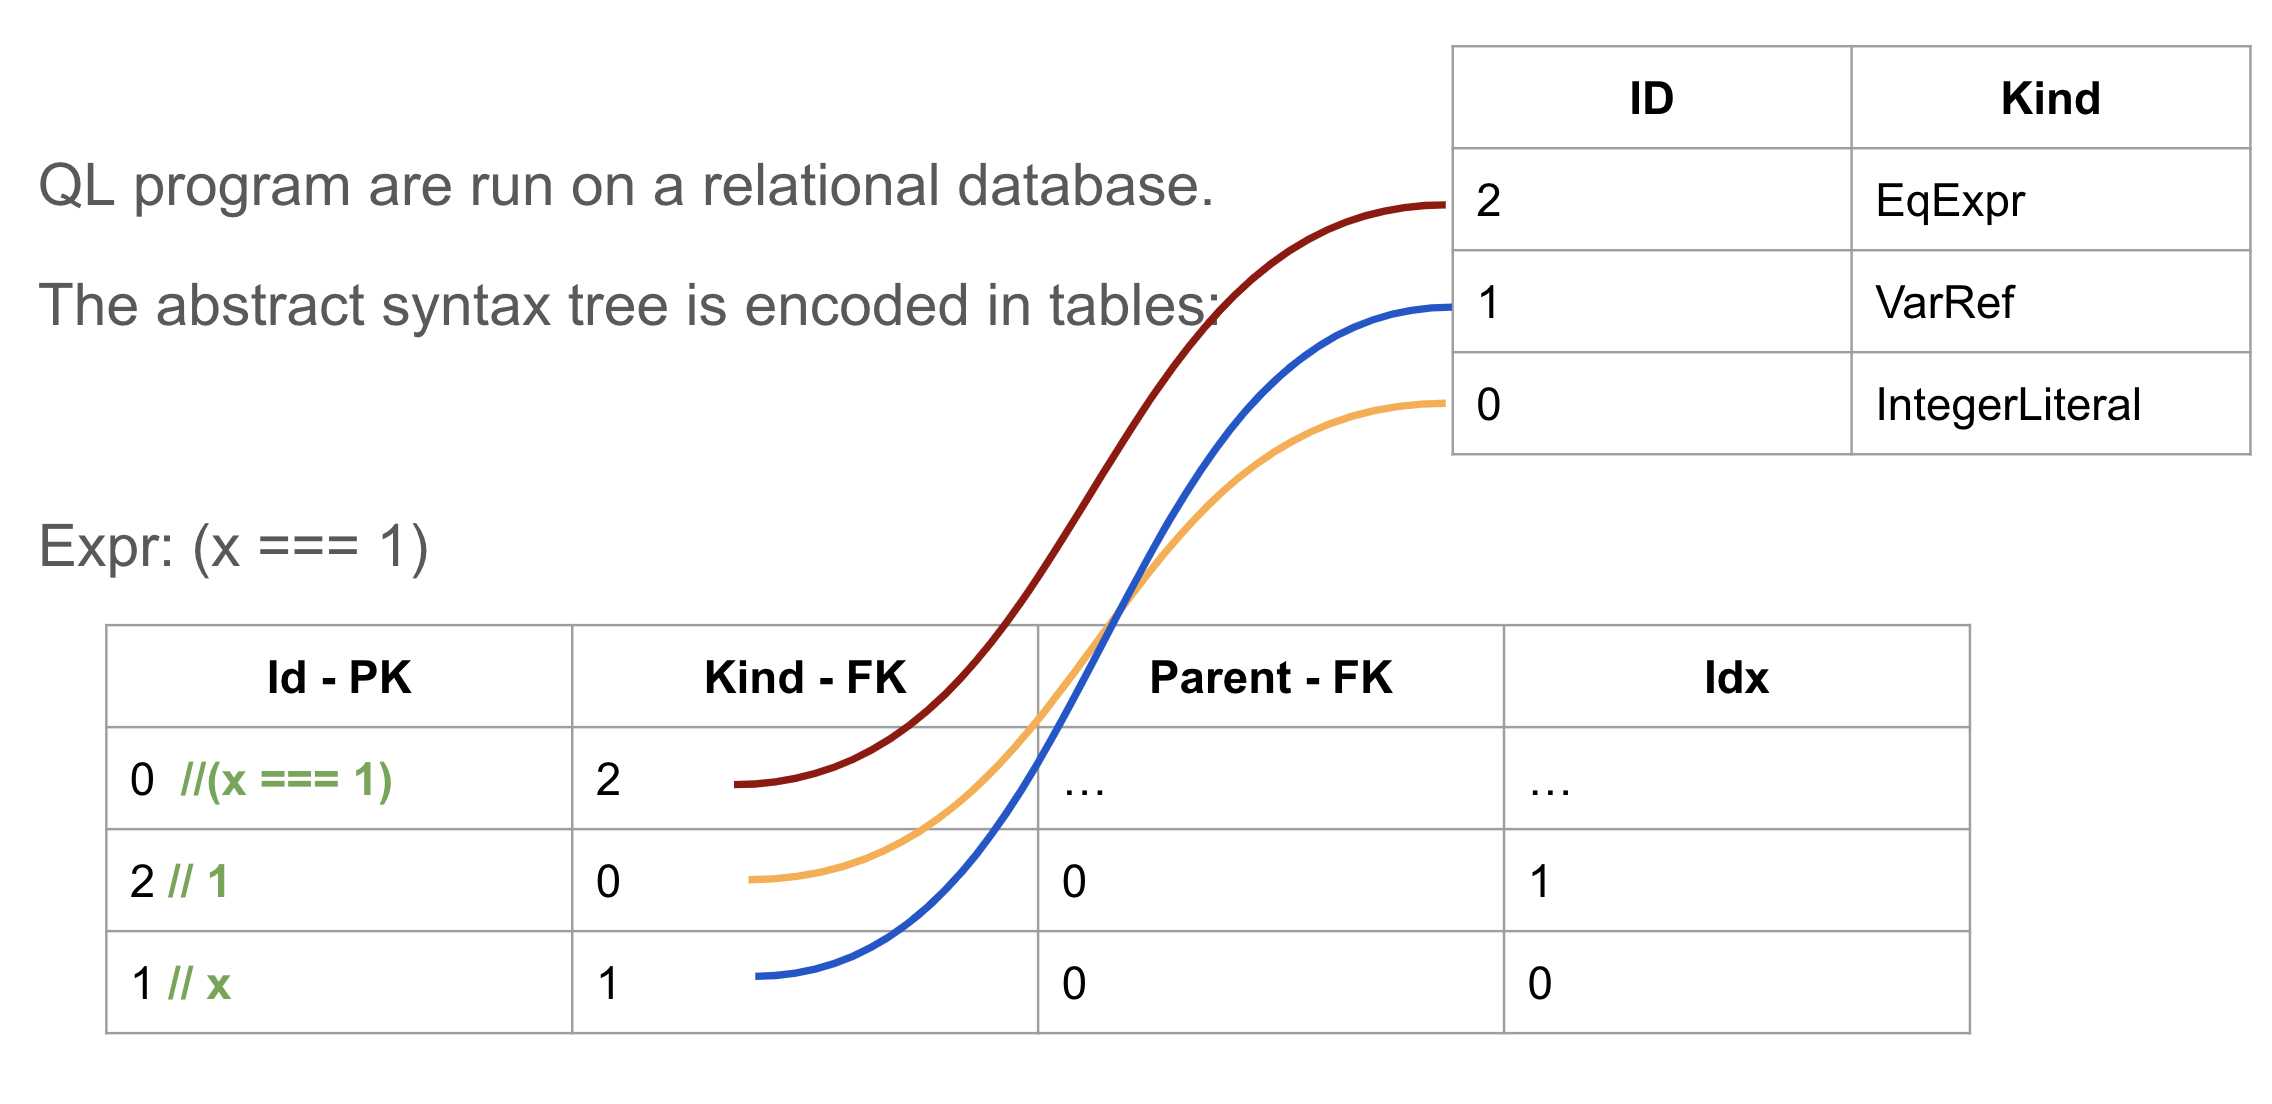
\includegraphics[scale=0.28]{img/storage}
\end{frame}

\begin{frame}[fragile]{Data Abstraction}
\begin{itemize}
\item QL classes hide the specifics of how data is stored in tables behind a higher-level interface, thereby acting like abstract datatypes.
\begin{lstlisting}[language=JastAdd]
class Expr extends @expr {
  Expr getParent() { exprs(this, _, result, _ ) }
  Expr getChildExpr(int i) { exprs(result, _, this, i) }
  string toString() { result = "expr" }
}
\end{lstlisting}
\item Easier to change data representation if all client analyses use \texttt{Expr} instead of directly accessing the DB.
\end{itemize}
\end{frame}

\begin{frame}[fragile]{Inheritance}
We can have a richer semantic interface by defining subclasses of Expr:
\begin{lstlisting}[language=JastAdd]
class EqExpr extends Expr {
  EqExpr() { exprs(this, 2, _, _) } // Characteristic predicated
  Expr getLeftOperand() { result = this.getChildExpr(0) }
  Expr getRightOperand() { result = this.getChildExpr(1) }
  string toString() { result = "===" }
}
\end{lstlisting}
\end{frame}
%
\begin{frame}[fragile]{Overriding}
As a practical example of overriding, consider implementing \textbf{Expr.isPure}:
\begin{lstlisting}[language=JastAdd]
class Expr extends @expr { predicate isPure() { none() }  //Built-in predicate that always fails

class Literal extends Expr { predicate isPure() { any() }  //Built-in predicate that always succeeds

class EqExpr extends Expr {
predicate isPure() { forall (Expr c | c = this.getChildExpr(_) | c.isPure()) //Propagating the check to all the children
 }
\end{lstlisting}

\end{frame}
%
\begin{frame}[fragile]{Interface vs Implementation}
We want to implement an analysis for JS to find comparisons between expressions with incompatible (dynamic) types, which will always evaluate to false at runtime

\begin{lstlisting}[language=JastAdd]
from EqExpr eq, Expr l, Expr r
where l = eq.getLeftOperand() and r = eq.getRightOperand() and incompatTypes(l, r)
select eq, "Operands have incompatible types."
\end{lstlisting}

\end{frame}

\begin{frame}[fragile]{Interface vs Implementation}
We want to implement an analysis for JS to find comparisons between expressions with incompatible (dynamic) types, which will always evaluate to false at runtime

\begin{lstlisting}[language=JastAdd]
from EqExpr eq, Expr l, Expr r, AnoterhKindOfExpr akoe ...
where l = eq.getLeftOperand() and r = eq.getRightOperand() and incompatTypes(l, r) or akoe ...
select eq, "Operands have incompatible types."
\end{lstlisting}
\end{frame}

\begin{frame}[fragile]{Interface vs Implementation}
\begin{itemize}
\item Let's define an abstract class
\begin{lstlisting}[language=JastAdd]
abstract class EqualityTest extends ASTNode {
abstract Expr getALeftOperand();
abstract Expr getARightOperand();
 }
\end{lstlisting}
\item Let's define two new classes:

\begin{lstlisting}[language=JastAdd]
class EqExprEqualityTest extends EqExpr, EqualityTest {
Expr getALeftOperand() { result = this.getLeftOperand() }
Expr getARightOperand() { result = this.getRightOperand() }
}

class SwitchEqualityTest extends SwitchStmt, EqualityTest {
Expr getALeftOperand() { result = this.getExpr() }
Expr getARightOperand() { result = this.getACase().getExpr() }
 }
\end{lstlisting}
\end{itemize}
\end{frame}

\begin{frame}[fragile]{Interface vs Implementation}
Now we can rewrite the query in terms of \texttt{EqualityTest}
\begin{lstlisting}[language=JastAdd]
from EqualityTest eq, Expr l, Expr r
where l = eq.getALeftOperand() and r = eq.getARightOperand() and incompatTypes(l, r)
select eq, "Operands have incompatible types."
\end{lstlisting}
\end{frame}

\begin{frame}{A study case}
\begin{itemize}
\item Reimplemented\textbf{ ErrorProne} in QL: 101 checks
\item One man-month of effort by experienced QL programmer
\item ErrorProne LOC: 10500 - 1100 (suggested fixes) - 2800 (import, packages and Override) = 6600
\item QL LOC: 2000 - 100 (imports) = 1900
\item Java implementation is 3.5x the size of the QL implementation
\item QL is 4 time slower than ErrorProne (Warm-up or steady state ?)
\item QL runs offline
\end{itemize}
\end{frame}

\begin{frame}{Conclusions}
QL is a lot of things and support many things:
\begin{itemize}
\item Data abstraction
\item Inheritance with dynamic dispatch
\item Overlapping classes
\item Relational member predicates
\item Object creation and mutation are not supported.
\item Parallelism comes for free
\item Conciseness
\item March 2016: Semmle's static analysis platform offers about 2500 individual analyses for 8 languages.
\end{itemize}


\end{frame}

%
%\begin{frame}[fragile]{Data Abstraction}
%
%\end{frame}








\end{document}